\documentclass[12pt, a4paper, titlepage]{article}

\usepackage{amsmath}
\usepackage[portuguese]{babel}
\usepackage{cite}
\usepackage{enumerate}
\usepackage[a4paper, margin=2cm]{geometry}
\usepackage{float}
\usepackage{graphicx}
\usepackage{hyperref}
\usepackage{setspace}

\chardef\_=`_

\title{\textbf{
    Investigação Operacional -- Trabalho Prático I  \\
    \large Problema de Empacotamento a Uma Dimensão
}}
\author{
    \begin{tabular}{ll}
        Ana Carolina Penha Cerqueira       & A104188 \\
        Humberto Gil Azevedo Sampaio Gomes & A104348 \\
        Ivo Filipe Mendes Vieira           & A103999 \\
        José António Fernandes Alves Lopes & A104541 \\
        José Rodrigo Ferreira Matos        & A100612 \\
    \end{tabular}
}
\date{23 de março de 2024}

\begin{document}

\onehalfspacing
\setlength{\parskip}{\baselineskip}
\setlength{\parindent}{0pt}
\def\arraystretch{1.5}

\maketitle

\begin{abstract}
    Este trabalho prático de Investigação Operacional tem como objetivo a resolução de um problema
    de empacotamento a uma dimensão utilizando o modelo de "um-corte", de Dyckhoff. \cite{dyckhoff}
    Em detalhe, procura-se a formulação do problema, a sua modelação, a sua resolução, e a validação
    do modelo construído.

	% TODO - adicionar que fizemos meta programação
\end{abstract}

\setcounter{section}{-1}
\section{Dados do problema}

Como exigido pelo enunciado, os dados do problema a resolver são determinados em função do número de
aluno mais elevado de entre os integrantes do grupo. No caso, este é A104541, que corresponde ao
aluno José Lopes, e dá origem aos seguintes dados:

\begin{table}[H]
    \begin{center}
        \begin{tabular}{c|c}
            Capacidade & Quantidade de contentores \\
            \hline
            11          & Ilimitada                 \\
            10          & 5                         \\
            7           & 5
        \end{tabular}
    \end{center}
    \caption{Número de contentores de cada comprimento disponíveis.}
	\label{containers-data}
\end{table}

\begin{table}[H]
    \begin{center}
        \begin{tabular}{c|c}
            Comprimento & Quantidade de itens \\
            \hline
            1           & 0                    \\
            2           & 13                   \\
            3           & 0                    \\
            4           & 9                    \\
            5           & 5
        \end{tabular}
    \end{center}
    \caption{Número de itens de cada comprimento para empacotar.}
	\label{items-data}
\end{table}

A soma dos comprimentos dos itens a empacotar é dada por:

$$2 \times 13 + 4 \times 9 + 5 \times 5 = 87$$

\section{Formulação do problema}

Pretende-se resolver um problema de empacotamento a uma dimensão, i.e., pretende-se determinar como
se deve distribuir um conjunto de itens por contentores. É necessário ter em conta que deve ser
atribuído exatamente um contentor a cada item, ou seja, um dado item não pode estar em mais do que
um contentor, e não pode haver itens que não tenham um contentor associado. Ademais, a soma dos
comprimentos dos itens em qualquer contentor não pode ultrapassar a sua capacidade.

Neste problema em específico, estão disponíveis contentores de capacidades 11, 10 e 7, sendo que há
contentores e capacidade 11 em número ilimitado, enquanto que há apenas 5 contentores de cada uma
das outras capacidades (tabela \ref{containers-data}). Pretendem-se empacotar 13 itens de
comprimento 2, 9 itens de comprimento 4, e 5 itens de comprimento 5 (tabela \ref{items-data}). O
objetivo é minimizar a soma das capacidade dos contentores utilizados.

% TODO - Descrever modelo de Dyckhoff

\section{Metaprogramação}

No modelo de um-corte, a expansão dos sumatórios da função objetivo e das restrições do modelo é,
por vários motivos, difícil de executar manualmente. Devido à grande dimensão dos sumatórios, o
processo não só é demorado, como também propício a erros de cálculo difíceis de diagnosticar: uma
solução errada ou a sua ausência apenas indica a existência de um erro, mas não a sua localização
no modelo. Ademais, a recriação do modelo teria de ser repetida caso os dados iniciais do problema
sofressem alterações, uma ocorrência constante no mundo real. Para endereçar este problema,
desenvolvemos \emph{scripts} em Python que geram o modelo LP automaticamente.

\subsection{Modelo do um-corte}

% TODO - Descrição do modelo dos um-cortes

\subsection{Modelo dos padrões de corte}

Inicialmente, o nosso grupo resolveu o problema de empacotamento proposto utilizando o modelo dos
padrões de corte, de modo a poder verificar a solução do modelo do um-corte quando este fosse
implementado. Também desenvolvemos um \emph{script} que gera este modelo automaticamente, cujo
funcionamento é descrito brevemente:

\begin{enumerate}[\hspace{1cm} \bfseries 1.]
	\item % TODO - descrição do modelo dos padrões de corte
\end{enumerate}

\section{Validação do modelo}

Após a criação do modelo de um-corte, procedemos à sua validação. Para tal, utilizamos o
\emph{lpsolve}, um programa para resolução de problemas de programação linear.
Após a execução do programa no output do \emph{script} python, obtivemos a seguinte solução:

\begin{table}[H]
    \begin{center}
        \begin{tabular}{c|c}
            Capacidade & Contentores utilizados \\
            \hline
            11          & 3                     \\
            10          & 4                     \\
            7           & 2
        \end{tabular}
    \end{center}
    \caption{Número de contentores utilizados.}
	\label{containers-used}
\end{table}

A partir da solução obtida, podemos concluir que a solução do modelo de um-corte é ótima, uma vez
que a soma das capacidades dos contentores utilizados é a menor possível, dado que corresponde ao
mesmo comprimento total dos itens a empacotar:

$$3 \times 11 + 4 \times 10 + 2 \times 7 = 87 \Leftrightarrow 2 \times 13 + 4 \times 9 + 5 \times 5 = 87$$

Além disso, ao descrever graficamente a solução obtida, podemos verificar que a solução é
efetivamente ótima:

\begin{figure}[H]
    \centering
    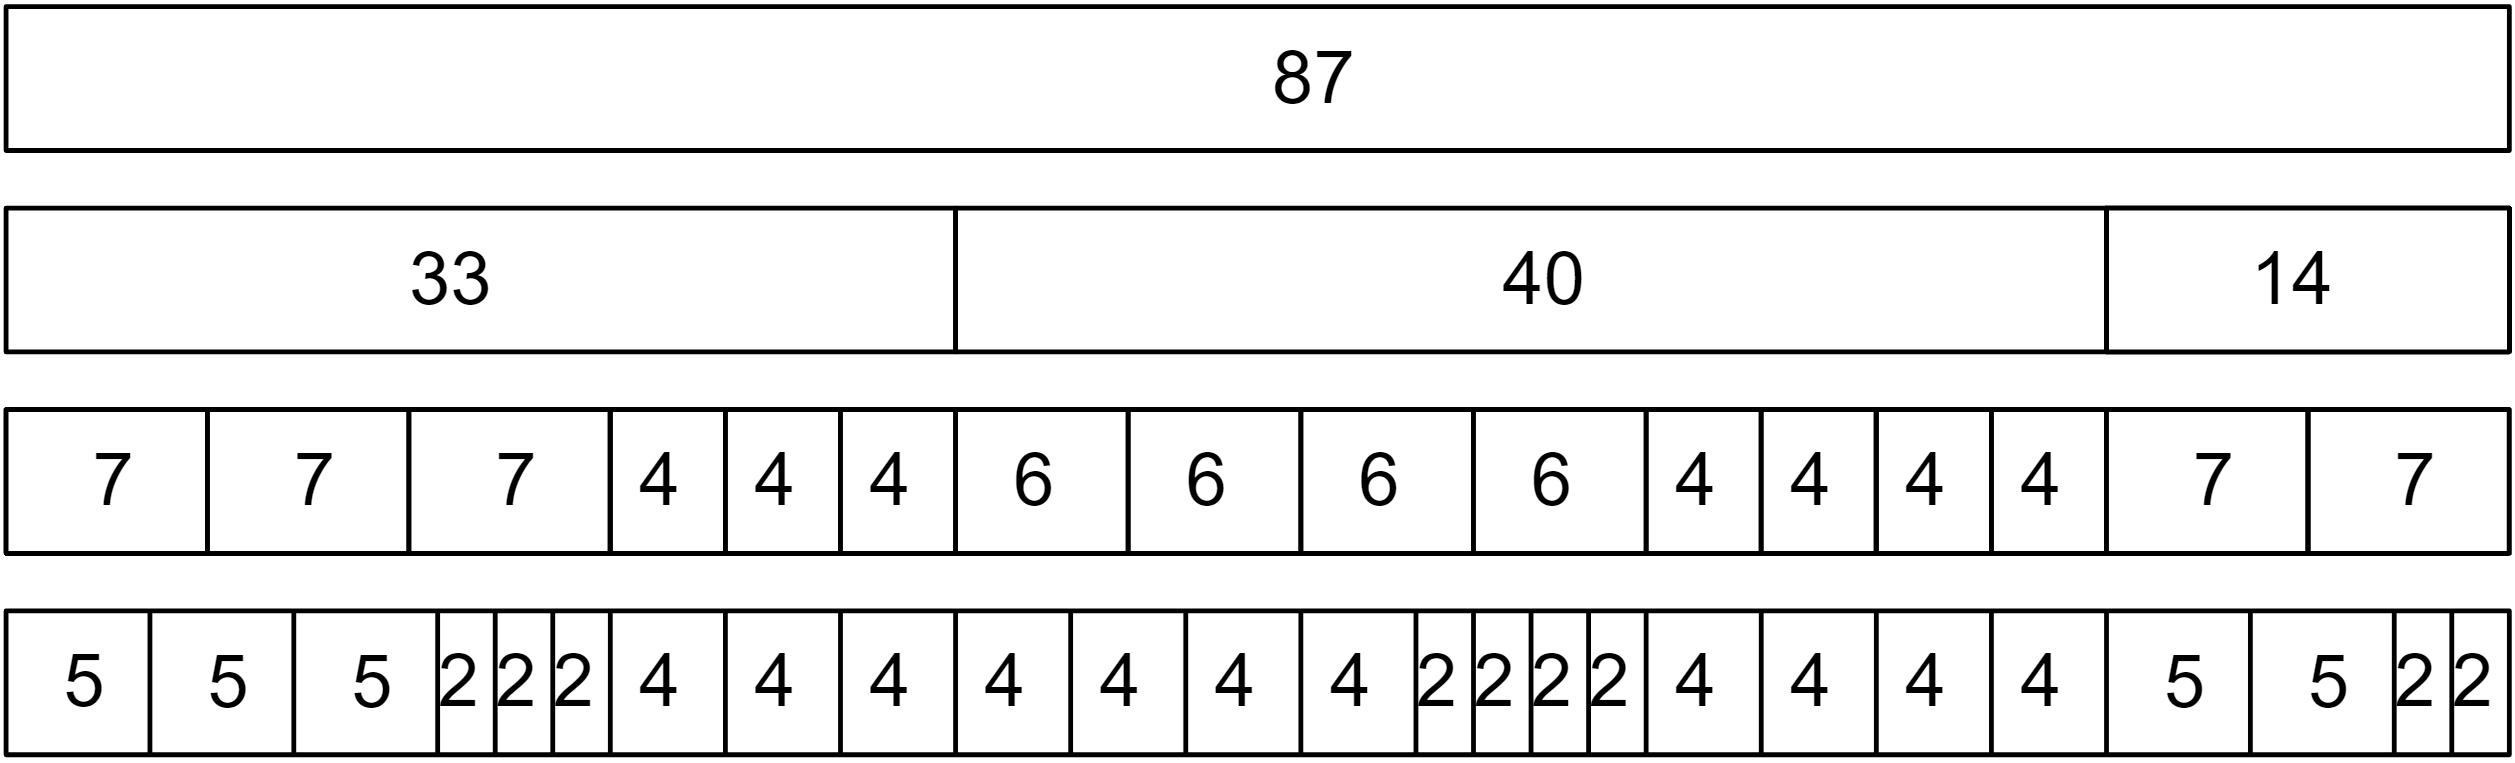
\includegraphics[width=0.75\linewidth]{images/cortes.png}
    \caption{Visualização dos cortes}
    \label{fig:cuts}
\end{figure}

% Isto é uma grande gambiarra, mas funciona para pôr a bibliografia como uma secção.
\section{Bibliografia}
\def\refname{}
\vspace{-1.5cm}
\begin{thebibliography}{9}
    \bibitem{dyckhoff}
    H. Dyckhoff, "A New Linear Programming Approach to the Cutting Stock Problem",
    \emph{Operations Research}, vol. 29, no. 6, Dec., pp. 1092-1104, 1981.
    \href{https://doi.org/10.1287/opre.29.6.1092}{doi: 10.1287/opre.29.6.1092}
\end{thebibliography}

\end{document}
